% Line styles, arrow tips, clipping, patterns, filled nodes with coloured
% text, a matrix of nodes, curves and a grid.
\documentclass{article}
\usepackage{tikz}
\usetikzlibrary{arrows.meta,patterns,shapes.geometric,matrix,decorations.pathmorphing}
\begin{document}
Line styles and more.

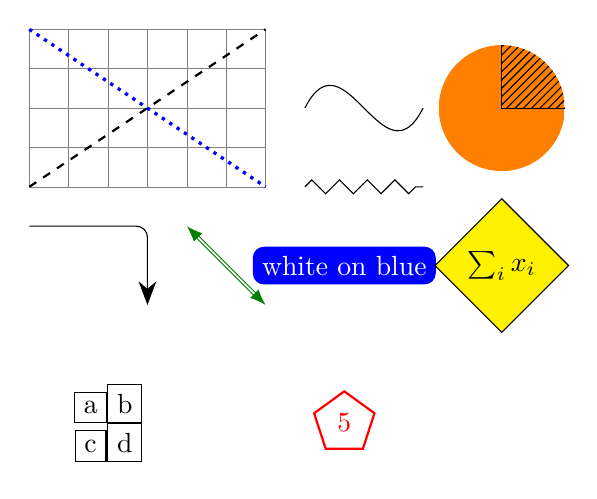
\begin{tikzpicture}
  \draw[help lines, step=0.5] (0,0) grid (3,2);
  \draw[dashed, thick] (0,0) -- (3,2);
  \draw[dotted, very thick, blue] (0,2) -- (3,0);
  \draw[-{Stealth[length=3mm]}, rounded corners] (0,-0.5) -- (1.5,-0.5) -- (1.5,-1.5);
  \draw[{Latex}-{Latex}, double, green!50!black] (2,-0.5) -- (3,-1.5);
  \draw[decorate, decoration=zigzag] (3.5,0) -- (5,0);
  \draw (3.5,1) .. controls (4,2) and (4.5,0) .. (5,1);
  \begin{scope}
    \clip (6,1) circle (0.8);
    \fill[orange] (5.2,0.2) rectangle (6.8,1.8);
    \draw[pattern=north east lines] (6,1) rectangle (7,2);
  \end{scope}
  \node[fill=blue, text=white, rounded corners] at (4,-1) {white on blue};
  \node[draw, diamond, fill=yellow] at (6,-1) {$\sum_i x_i$};
  \matrix[matrix of nodes, nodes={draw}] at (1,-3) {a & b \\ c & d \\};
  \node[regular polygon, regular polygon sides=5, draw, thick, red] at (4,-3) {5};
\end{tikzpicture}
\end{document}
